\label{chap:lit}
In this chapter we shall discuss background literature relating to the aims of this project as
having a good understanding of the work of others and the motivations for their work will provide
a basis for the work undertaken in the project.

\section{Flux}
The photon mapping algorithm is based around emitting photons from light sources, the unit of measurement of a photon is
Radiant flux $\Phi$ the exact definition of flux is not relivant to the disscussion, but is essentially a measurement
of radiant energy with respect to time \cite{JensenBook}.

\section{Radiance}
Radiance commonly referers to two quantities, incident radiance and exitance radiance, incident radiance being the radiance
that fall on a surface, exitance radiance being radiance from a surface (either from reflection or emission)


\section{The BDRF}
\label{sec:bdrf}
Most global illumination systems need to describe the radiance from an object, this includes the
reflected radiance by an object from the scene.
The bidirectinoal reflectance distribution function \cite{Nicodemus65}is a function that describes 
the reflectance of a surface at point $x$ with respect to an outwards direction $\omega_{o}$, and 
inwards direction $\omega_{i}$. The BDRF is commonly written as $f_{r}(x, \omega_{i},\omega_{o})$. 
The BDRF is a vital part of computer graphics as it describes the reflectance of a surface which is 
vital in global illumination as we need to consider reflectance from all objects in a scene.

The BRDF is a mesure of the outgoing radiance $L$ in a given direction $\omega_{o}$ from an incoming
irradiance $E$ from a direction $\omega_{i}$. The BRDF for a surface is given by:

\begin{equation}
f_{r}(\omega_{i}, \omega_{o}) = \frac{L_{\omega_{i}}}{E_{\omega{o}}}
\end{equation}

An example of a simple BDRF would be that of Lambertian reflection whereby the light is reflected
in all directions equally, the BRDF for this is:

\begin{equation}
f_{r}(\omega_{i}, \omega_{o}) = \frac{\rho}{\pi}
\end{equation}

Where $\rho$ is the reflectivity of the surface, for physically based rendering this is a real
number between zero and one.

For the system that I am developing it is important to be able to specify the material of an
object in the scene in a flexible manner, this will include a method of representing the BDRF of
an object that can be easily configured.

\section{The Rendering Equation}
Central to most modern rendering systems is the rendering equation, the rendering equation is an
approximation to the light transfer of a scene \cite{Kajiya86}. A frequency independant version of
the rendering equation is given below.

\begin{equation}
L_{r}(x, \omega_{o}) = L_{e}(x, \omega_{o})
					 + f(x)
					   \int_{\Omega}
					 		f_{r}(x, \omega_{i}, \omega_{o})
							(\omega_{i} \cdot n)d\omega_{i}
\end{equation}
Where $L_{r}$ is the radiance from the surface at point x, $L_{e}$ the emmited radiance from the
surface and $f_{r}$ is the BDRF as described in section~\ref{sec:bdrf}.

There have been many developments within computer graphics that attempt to find approximations
to the rendering equation, radiosity \cite{Goral85}which attempts to find the solution by splitting 
the geometry of a scene into smaller patches and builds a system of linear equations that solve the 
radiosity value for the patch, this technique is simple but sufferes from some problems, for one it 
is only able to account for lambertian diffuse reflections from other object and so cannot be used
to render specular reflections. Radiosity is still used within architectural applications as the
radiometry is view independant and as such is well suited to applications such as walk-throughs.
Monte-carlo methods are another method that is more general that radiometry, this method is a
stocastic method that attempts to find the solution of the rendering equation by sampling the light
transfer of a point untill a adequete approximation is found, a common form of this is distributed
raytracing whereby raytracing as introduced by Whitted \cite{whitted79a} is performed but for each
intersection the choice of reflecting, refracting or absoring is taken from a distribution as the
number of rays emmited increases the image converges to the solution of the rendering equation.

Understandind the motives of the rendering equation will be vital if I am to be sucsessfull in
developing a photon mapping system, the solution that most rendering algorithms produce are an
approximation to the rendering equation and as such will be the focus of my system.


\section{Path Notation}
The radiance estimate on the right hand side of the rendering equation is typically evaluated by a recursive call to the
procedure that evaluates radiance at a point in the direction $\omega'$, as we perform more evaluation we create a path
from the eye to the final destination of the ray, it is frequently convienient to refer to these paths by the interaction
that the ray has with surfaces along the path, we use a regular expression language to express these paths, tokens in the
language include:
\begin{description}
\item[E] The eye or camera
\item[D] A diffuse surface
\item[S] A specular surface.
\item[L] A light
\end{description}

Paths begin with the eye and end at a light, a full solution to the rendering equation will evaluate the radiance due
to all paths \textbf{E(S\textbar D)*L}, raytracing evaluates all paths \textbf{ES*DL}

\section{Raytracing}
\subsection{Pixel Sampling}
As the raytracer is performing distribution raytracing each thread will perform multiple raytracing operations for each pixel
that it processes each sample per pixel is offset inside the pixel to perform antialiasing, this reduces the sharp edges that
can be seen in images. In order to improve the appearence of the image we also perform jittering on the samples this reduces
certain artifacts such as banding. \todo{Make sure the banding comment is correct and if so find a reference for it}

\missingfigure{anti-aliasing}

\subsection{Intersection Tests (0.5 pages)}
Intersection tests are another vital part of any raytracer. a number of intersection tests are needed, I will not include
an extensive treatment of the intersection tests mearly a listing of the most notable used.

\begin{description}
\item[Triangle] Moller-Trumbore intersection test \cite{MolTru97}
\item[AABB]
\item[kD-tree] As described in TODO:
\end{description}

\subsection{volume intersection}
Unlike intersection with all other object types the intersection with a participating media is non deterministic, this is
due to the fact that the intersection of the ray is determined by the extinction coefficient which gives a probablilty
of interaction, the depth of the interaction is calculated with equation \todo{add equation}, performing this non-deterministic
intersection test allows for objects within the medium to be interacted with when performing ray-marching.

\missingfigure{Non-deterministic intersection test}

\subsection{Intersection Storage}
When raytracing the scene the intersection point of the ray needs to be calculated and stored, this will include data that
is specific to an objects intersection, for example an intersection with a triangle mesh will need to record the trangle
that was intersected and as a result will need to record the barycentric coordinate at the point of intersection.

\subsection{Scene Traversal}

\section{Shading}

\subsection{Direct Illumination}
\subsubsection{Texture Mapping}
Performing texture mapping requires the ability to query the texture coordinates at a point of intersection, for mesh objects this
will interpolate the barycentric coordinates for the triangle of intersection, spheres use a spherical mapping that uses the
spherical coordinates to generate u,v values.

\subsection{Specular Reflection and Transmission}

\subsection{Nearest Neighbour Search}

\subsection{Diffuse Interreflection}
While it is possible to estimate the contribition to the radiance at an intersection point directly from the photon map this
approach can cause visual artifacts due to variance in the estimate in order to reduce these artifacts we perfom a final gather
stage at the point of intersect that produces a diffuse ray that is traced into the scene until a non-specular object is intesected,
we then perform the radiance at this point and use this information to estimate the radiance incident at the original point of intersection.
In order for the final gather to produce a correct estimate of the radiance we need to perform this stage multiple times per pixel, as we
are performing distributed raytracing this is a trivial addition. When calcualting the radiance for the final gather it has been shown \todo{cite}
that if the distance of the final gather point is lower than some threshold perfoming an additional diffuse bounce reduces errors at geometry
such as sharp corners where the radiance estimate can be inaccurate due to accounting for photons not truly at the surface.

\begin{figure}
\centering
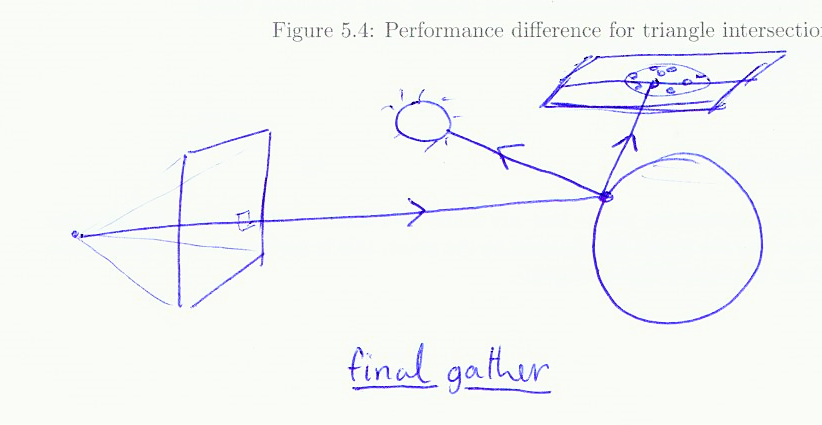
\includegraphics[width=\textwidth]{./images/final_gather.png}
\label{fig:final_gather}
\caption{Final Gather}
\end{figure}

\subsection{Caustics}

\subsection{Participating Media}

In the case of a ray that intersects a participating media before intersecting a surface we need to calculate three components to
the radiance along the path of the ray in the medium, these are single scattering direct illumination, multiple scattering (in-scattering)
and attenuation (out-scattering)

\subsubsection{Ray Marching}
In order to evaluate the radiace from the participating media we perform a ray-march, this is an iterative operation that evaluates the
radiance along the ray as it moves through the participating media.

\begin{equation}
L(x, \omega) = \sum\limits_{i = 1}^N L^l(x, \omega_l')p(x, \omega_l', \omega)\sigma_s(x)\Delta x + e^{- \sigma_t \Delta x} L (x + \omega \Delta x, \omega)
\end{equation}

\subsubsection{Attenuation}
As a ray travels through a medium the radiance can be reduced due to out-scattering and absortion, this can be calculated by evaluating
the integral given in equation \todo{Add the equation}, as we are only considering homogeneous participating media this can be
simplified as the properties being integrated are constant and a closed form solution is possible.

\missingfigure{Attenuation Equation}

\subsubsection{Direct Illumination}
At each point in the ray march we also evaluate the contribution from each light in the scene due to single scattering, this is performed
by performing an additional ray march in the direction of the light and evalute the radiance arriving at the point on the ray.

\subsubsection{Muliple Scattering}


\input{./LitReview/monte_carlo.tex}
\section{Photon mapping}
Photon mapping was first developed by Jensen \cite{Jensen95b} as an extension to the traditional ray
tracing algorithm proposed by Whitted \cite{whitted79a} whereby a preprocessing step is added that
creates a photon map of the scene.

The photon mapping algorithm begins by emitting photons from each light source in the scence until
the photon is absorbed by a diffuse surface within the scene, each of the photons absorbed are stored within a photon map
which is an efficient data structure that will store information about the photon such as the
location of the absorbtion, the direction from which the photon was traveling and the photons
energy. the photon map is a spatial structure as we will query the photon map for the photons
within a location as such it is common to store the photon map in a kd-tree to allow an efficient
nearest neighbour search.

Different types of photon maps are used with different accuracies in order to
improve the efficiency, for instance in \cite{Jensen96a} two photon maps are used, a global photon
map and a caustic photon map, the caustic photon map contains photons that arrive at a location from
either the specular reflections or refractions , this photon map is stored at a higher
accuraracy as its data will be visulaised directly to produce the apperance of caustics in an image.

The general photon map contains all other types of photons stores, such as direct and indirect
illuminations and shadow photons as described in \cite{Jensen95c, Jensen96a} these shadow photons
allow for the number of shadow rays to be reduced as we do not need to shoot shadow rays if the
photon search returns only shadow photons.

The second stage in the photon mapping algorithm is the raytracing stage, this state is simalar
to the algorithm in \cite{whitted79a} but we now have the data stored within the photon map to make
use of. Rays are shot from the eye into the scene until an intersection is found, we then use
the propertiyes of object hit and the photon maps to calculate the colour set for the pixel, this
is done by estimating the radiance at the point of intersection, a nearest neighbor search is
performed on the photon map cetererd at the point of intersection, the radius of the search is
increased until the number of photons has reached a predetermined number $n$, the estimate of the
radiance is then given by the sum of the radiances of the photons within the search.

\begin{equation}
\label{eq:radiance_disk_estimate}
L_{r}(x, \vec{\omega})
\approx
\sum_{p=1}^n
f_{r}(x,\vec{\omega}_{p}', \vec{\omega})
\frac
{
	\Delta\Phi_{p}(x, \vec{\omega}_{p}')
}
{
\pi r^{2}
}
\end{equation}

The radiance is estimates as the density of a disk of radius $r$, this estimate is used as it is
assumed that the photons within the search will lie on the surface of the object and locally 
relitivly flat, this is accounted for by the division of $\pi r^2$ term in equation~\ref{eq:radiance_disk_estimate}.

The density estimate given in \cite{Jensen96a} can produce poor results in the case of geometry with
areas that are close together but not flat, such as the corners of a room, in this case the
estimate of the radiance will be too high as the photons lying on the other wall will contribute to
the estimate, a solution to this is given in \cite{JensenBook}, where the search radius is flattened along
an axis orthoganol to the normal of the surface. I am not sure if the computational cost of this
is worth the effort as more photons can be emmited which will increase the photon density thus
decreasing the search radius.

\section{Participating media.}
Participating media are materials or objects that interact with light within the surface of the
object, these interactions can create interesting visual effects that add to the realism of a 
scene, a good example of participating media would be smoke, as light enters smoke it will
experience scattering that will cause the path of the light to be altered. \cite{Blinn82}
In order to render participating media a solution to the volume rendering equation must be found,
this equation describes the light transfer within the participating media, Jensen presents a
good explination \cite{JensenBook}.

Participating media are generally split into two types, inhomogenios and homogenios, this describes
if the properties of the participating media are constant, an example of a
participating media that is homogenios would be a liquid such as milk, an example of a
non-homogenios media woulf be smoke as the density of the smoke (and as a result how much it scatters
light) is not constant.

Early work in this area include work done by Blinn \cite{Blinn82}, in this paper a model for the
scattering in clouds and other such media is given, this paper only considers single scattering
in its approximation and as noted in \cite{Jensen98} only suitible for optically thin media.

\subsection{Volume ray casting}
Volume ray casting is a technique that is central to participating media as it allows rays to be
seen as moving through a media, this is apposed to traditional raytracing where the ray will only
interact at the point of intersection of an object. In ray casting the ray is "marched" through
the medium, at each step in the process a calculation can be performed in order to decide if an
action should be taken (i.e in or out scattering)

\subsection{Volumetric Photon Mapping}

One of the earliest applications of photon mapping to render participating media was \cite{Jensen98}
in this paper the concept of volumetric photon mapping and the volume photon map was introduced,
this photon map allows the interaction of light within a participating media to be taken into
account, this could be one of the following, in-scattering, out-scattering, absorbsion or emmission.
The volume map is a seperate map to the surface map usually used in the photon mapping algorithm,
this is because the desity estimate is different as the sample of photons are taken from the volume
enclosing $n$ photons and not the disk. The technique in this paper deals with the case of 
homgenious and non-homogenious media as the volume map decouples the representation of the radiance 
from the geometry of the media.

Building the volumetric photon map is different to that of the surface volum map as the photons
can interact anywhere within the definition of the volume, there is defined for the volumne a
cumulatice probablility density function that defines the probability of an interaction at all
points $x$ within the volume.

\begin{equation}
F(x) = 1 - \tau(x_{s}, s)
\end{equation}

where $\tau$ is the transmittance which is computed by ray marching.

\begin{equation}
\label{eq:radiance_volumn_estimate}
L_{r}(x, \vec{\omega})
\approx
\frac
{1}
{\sigma(x)}
\sum_{p=1}^n
f_{r}(x,\vec{\omega}_{p}', \vec{\omega})
\frac
{
	\Delta\Phi_{p}(x, \vec{\omega}_{p}')
}
{
\frac{3}{4} \pi r^{3}
}
\end{equation}

\subsection{Sub Surface Scattering}
Sub surface scattering is caused by a class of participating media where the light transport of the
material can be approximated by a function whereby the reflection of light at a point $x$ is
reflected at another point $x'$ This causes a softening of the apperance of the material a common
example of this is the human skin where a large amount of the reflected light by the skin undergoes
some amount of sub surface scattering. The reason that this case of participating media is
seperated from the general class is that their are specific properties of SSS that allow for
the calcualtion of the light transport more efficiently. Subsurface scattering can be described by
the bidirectional surface scattering function BDSSRF \cite{Jensen01}, this is a generalisation of 
the BDRF and is given as:

\begin{equation}
\label{eq:bdssrf}
	S(x_{i}, \vec{\omega}_{i};x_{o}, \vec{\omega}_{o}) =
		\frac
		{ dL_{o}(x_{o},\vec{\omega}_o)}
		{d\Phi_{i}(x_{i}, \vec{\omega_{i}})}
\end{equation}

From Equation~\ref{eq:bdssrf} it can be seen that their are two points that needed to form the
BDSSRF, the incidence location $x$ and the reflectance location $x'$, this can be seen as the
light incident to $x$ being scattered within the surface of the material and being reflected at
the point $x'$. The BDRF can be seen as a special case of this function where their is the
assumption that the location of emmited radiance is the same as that of incidence irradiance.

\input{./LitReview/volumetric_pm.tex}
\section{Photon mapping advances}
Since the initial creation of the photon mapping algorithm in 1996 there have been many improvements
and modifications to the photon mapping algorithm in order to increase the efficiency and the
range of effects that can be visulised.

\subsection{Reverse Photon Mapping}
In order to speed up the photon mapping algorithm Havran et al. developed the reverse photon mapping
algorithm, it is claimed in his paper that substantial speedups are possible by performing the
raytracing stage before the photon mapping stage by accessing memory in a more coherent manner.

\subsection{Progressive Photon Mapping}
Progressive Photon Mapping \cite{Hachisuka08} is a reformulation of the photon mapping algorithm
into a multipass solution to the rendering equation in which the raytracing stage is performed prior
to the photon mapping stage in a simalar way to reverse photon mapping.

In the traditional photon mapping algorithm the number of photons that are emitted into the scene
are fixed, as such it is not possible to obtain an estimate of the radiance to an arbitrary
precision, this can cause the estimate of the radiance to be blured. Progressive photon mapping
attempts to solve this problem by performing more than one photon mapping pass. After each photon
map stage the search radius at each pixel is reduced, this allows details to be refined through
subsequent passes. In addition to the ability to refine the image quality the memory requirement to
produce an image to a given precision is reduced as each photon map does not need to be stored in
main memory.

While this algorithm has been shown to be a useful addition to the traditional photon mapping
algorithm it is much more complicated, we need to perform more than one photon mapping stage which
require the radiance estimate to be recalculated multiple times.

\subsection{Stochastic PPM}
Stochatic Progressive Photon Mapping (SPPM) \cite{Hachisuka09} is a recently extension to PPM that
is simalar in motivations as distributed raytracing, that is to be able to use the algorithm to
produce phenomena such as depth of field, motion blur and glossy reflections. This method has been
shown to converge to the correct solution for these phenomena and specular-diffuse-specular paths
faster that normal PPM.

\subsection{Dynamic Scenes}
Although the photon mapping algorithm has traditionaly been used for static scenes there has
recently been work towards modifiing the algorithm so that it can be used for dynamic scenes, the
work of Weiss et al. \cite{Weiss12} in this paper it presents a method of rendering that uses
information from previous frames of the scene in order to gain a speedup of the rendering process.

\section{Acceleration Structures}
In order to produce an image of a non-trivial scene accelerating structures are a nessesity, the
amount of time to check intersections for each ray grows with order  $O(N^2)$ if each object is
checked for an intersection. Some candidates for structures are, Octrees, KD Trees, BSP trees. All
of these data structures are designed to decrease the amount of time spent checking for 
intersections. It may be worth an investigation the performance characteristics of the various
data-structures within the system, this can easily be done by making the underlying implementation
of the data-structure transparent to the rest of the system.

\subsection{KD Trees}
A kd-tree is a data structure that partitions space along split-planes which are axis aligned
hyperplanes first preposed by Bently \cite{Bently75}.
The use of kd-trees in rendering applications is common as they reduce the time
required to find the intersection of a ray and an object within a kd-tree. kd-trees are also needed
within the photon mapping algorithm for the radiance estimate as we need to perform a
neighbour search, Jensen uses this data structure within his implementation of the photon mapping
algorithm in his book \cite{JensenBook}.

\subsection{Building KD-Trees}
Wald desribes an algorithm for building a kd-tree in $O(N log(N))$ \cite{Wald06}, as stated in his
paper the desire for more and more complex scenes requires that attention should be make to the 
building of the kd-tree as it can begin to take substantial amount of computing resources to
perform. This paper is a good overview of techniques for building a kd-tree.

\subsubsection{Surface Area Huristic}
The Surface Area Huristic (SAH) is a technique often used in the building of kd-trees in order to
decide upon the location of the split plane. First presented by MacDonald et al. \cite{MacDonald90}
the SAH estimates the cost of splitting at a given point on a kd-tree, this is done by estimating the
cost of traversing the structure and the probability of a ray intersecting the objects within the
structure. The SAH does make some assumptions such as the cost of traversel etc, as noted in
\cite{Wald06} some of these assumtions are not strictly correct but the result of using the SAH
are still valid.

\subsection{Nearest Neighbour search}
In order to produce a radiance estimate for a location on a surface we need to be able to query to
photon map in order to find the nearest n photons, the kd-tree is a good candidate for this search
as it is possible to perform the search in $O(log(N))$. The algorithm was first proposed in the
paper introducing kd-trees by Bently \cite{Bently75} although as noted by Bently in later versions of
the paper a more clear explination of the algorithm is stated by Freidman et al. \cite{Freidman77}.

\subsection{Ray KD-Tree Traversal}
Devoting time to creating efficient traversal algorithms is vital for all applications that
include raytracing as a large proportion of the running time will be used performing these
intersection tests, Fussell \cite{Fussell88} describes an algorithm to perform this traversal that
performs front to back search of the enclosing volumes allowing the closest intersection to be found
efficiently.

\subsection{Irradiance Caching}
Along with the photon map, irradiance caching is a strategy to reduce the computation in order to
produce a correct image, developed by Ward et al. \cite{Ward88}. The algorithm stored irradiance
values calculated on lambertian diffuse surfaces in a data structure that allows for the values
to be interpolated for other points on the surface, this is done with the assumption that the
values will be slowly varing over the surface. A thorough explination of irradiance caching with
respect to photon mapping can be found by Jensen \cite{JensenBook}

